\chapter{\xlabel{pol2_dr_theory}POL-2 Data Reduction -- The Theory}
\label{sec:dr}
\section{\xlabel{dataflow}The Data Flow}

POL-2 data reduction is an involved process. A broad overview of this
process is presented here first, followed by a discussion of the specific
details. It should be noted that this same procedure is used irrespective
of whether single or multiple observations are to be reduced.

The following description assumes that the \task{makemap} command is
being used to create maps. \cref{Section}{sec:skyloop}{SKYLOOP} explains the effects
of using the \task{skyloop} command in place of \task{makemap}.

The data reduction process can be broken down into three main stages --
referred to as ``Run 1'', ``Run 2'' and ``Run 3'' in
\cref{Figure}{fig:pol2drflow}{}.

\begin{figure}[t!]
\begin{center}
\latexhtml{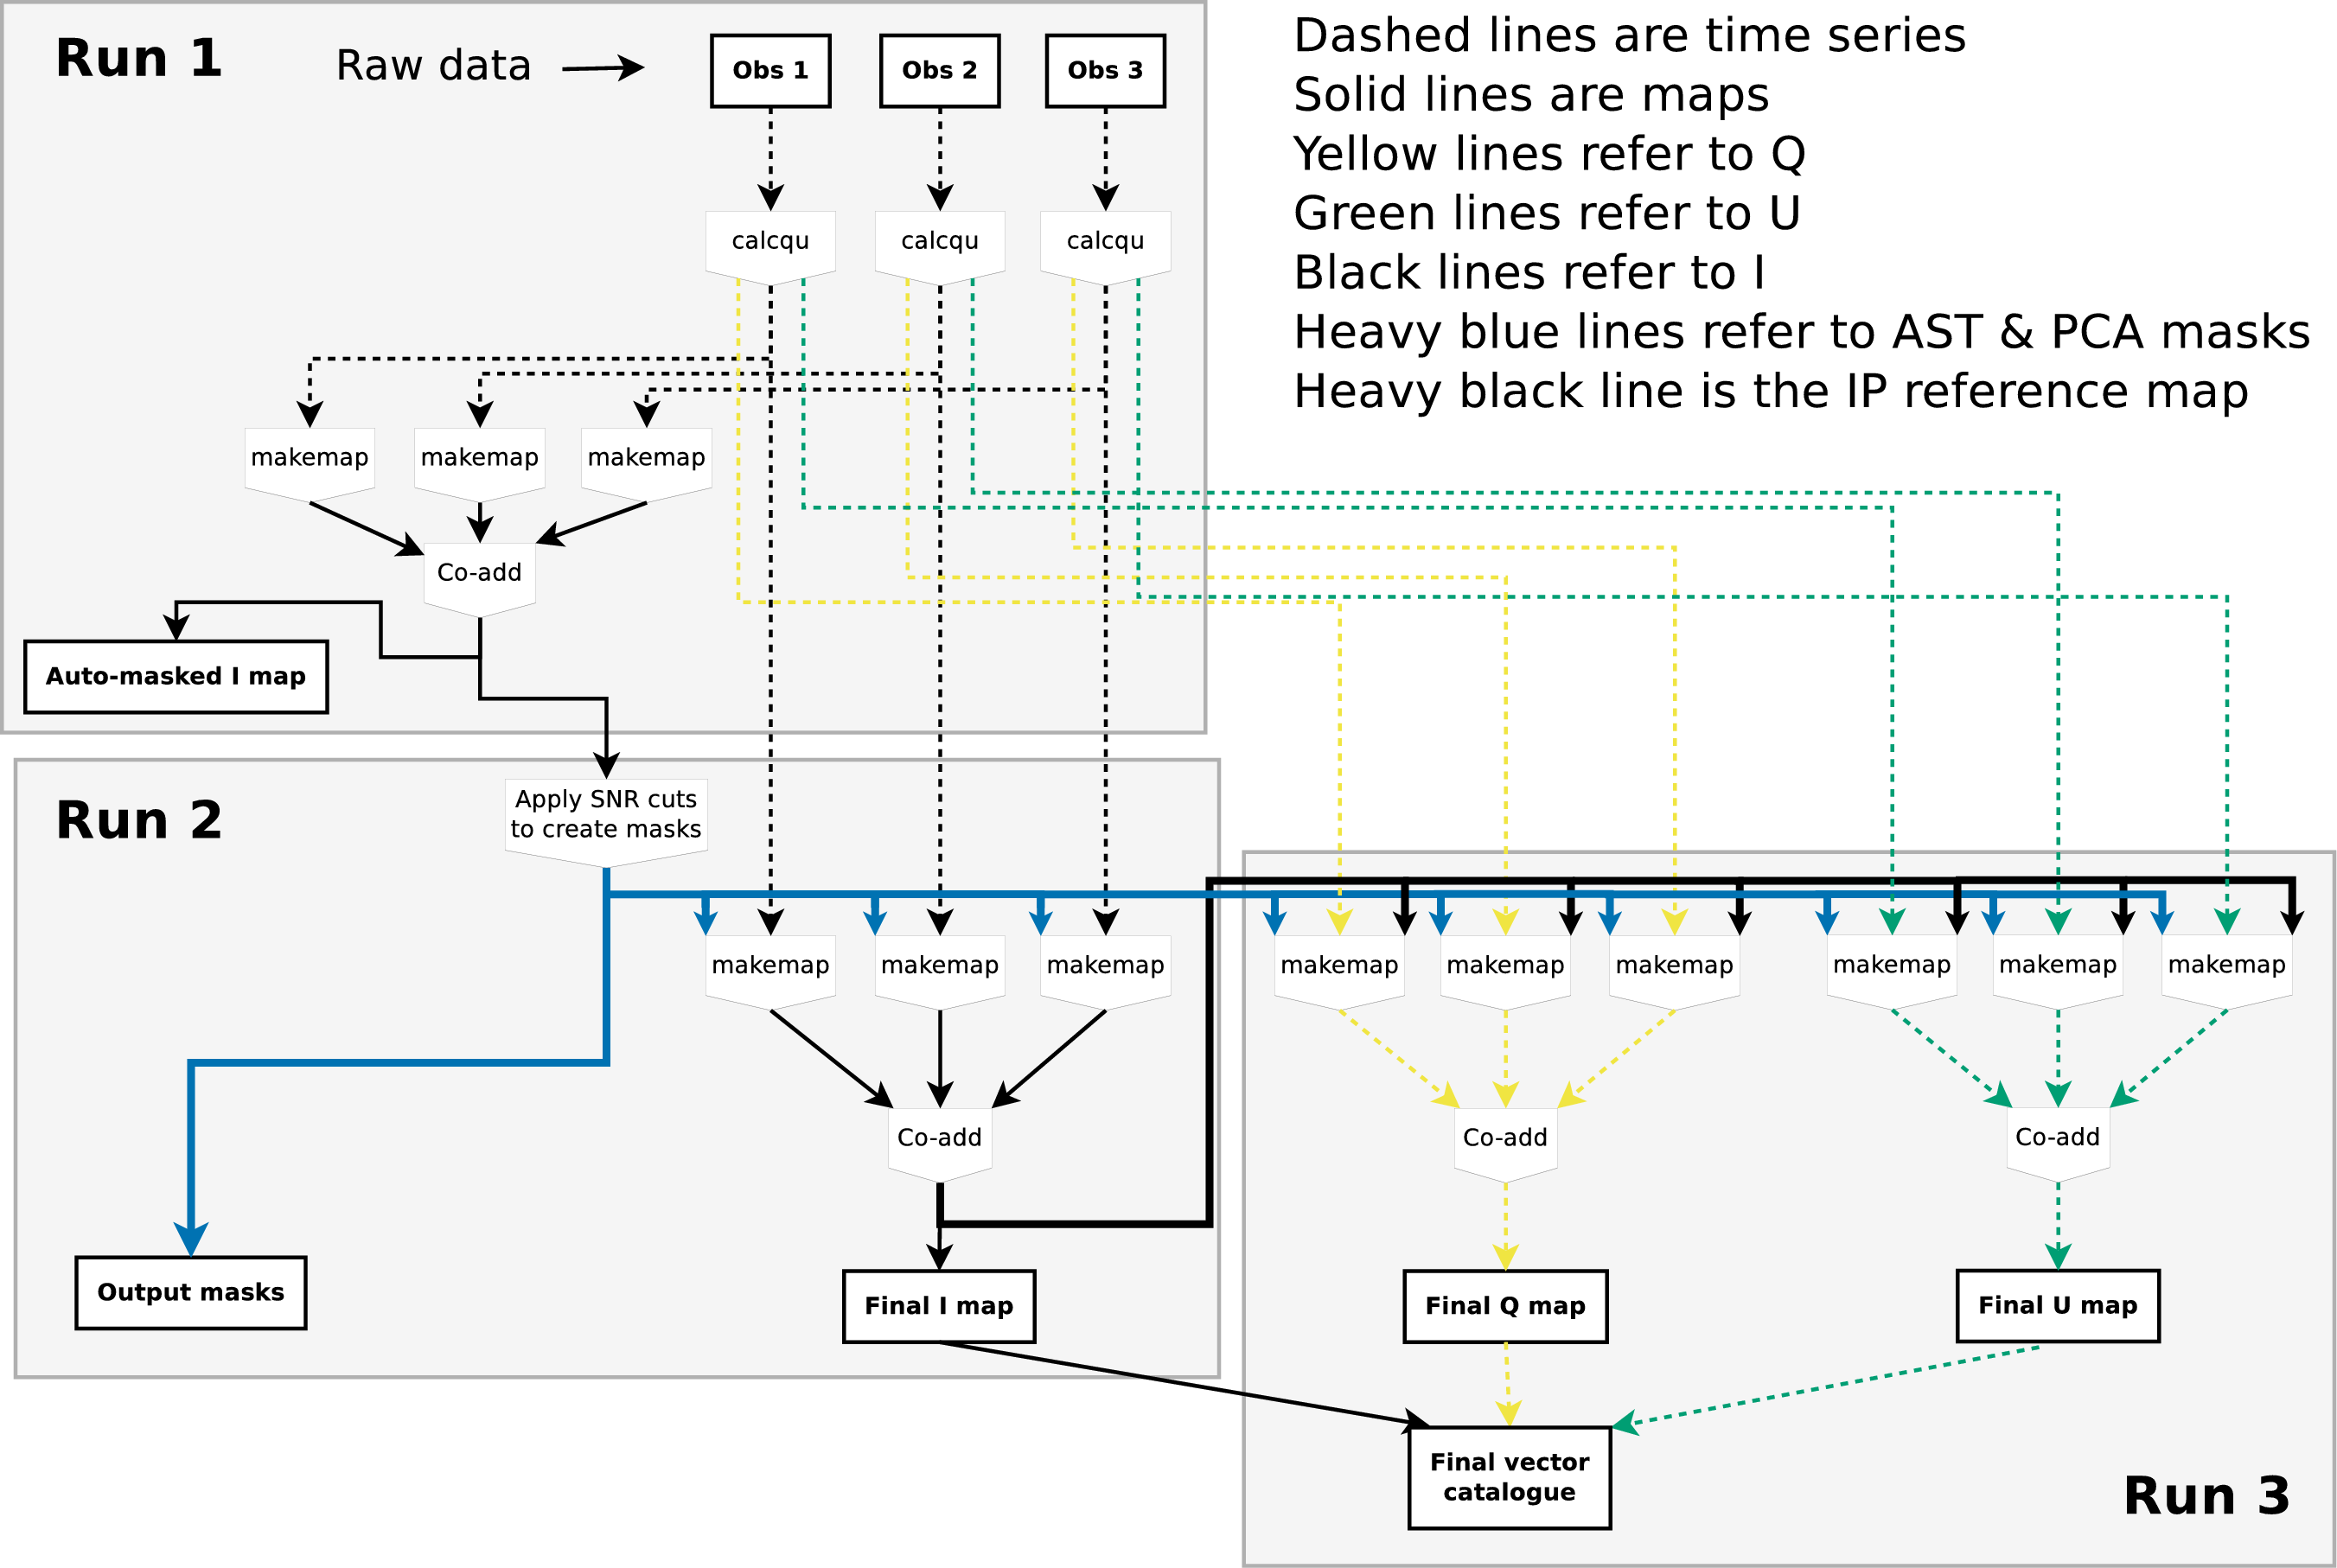
\includegraphics[width=1.25\linewidth,angle=90]{pol2map_flow}}{
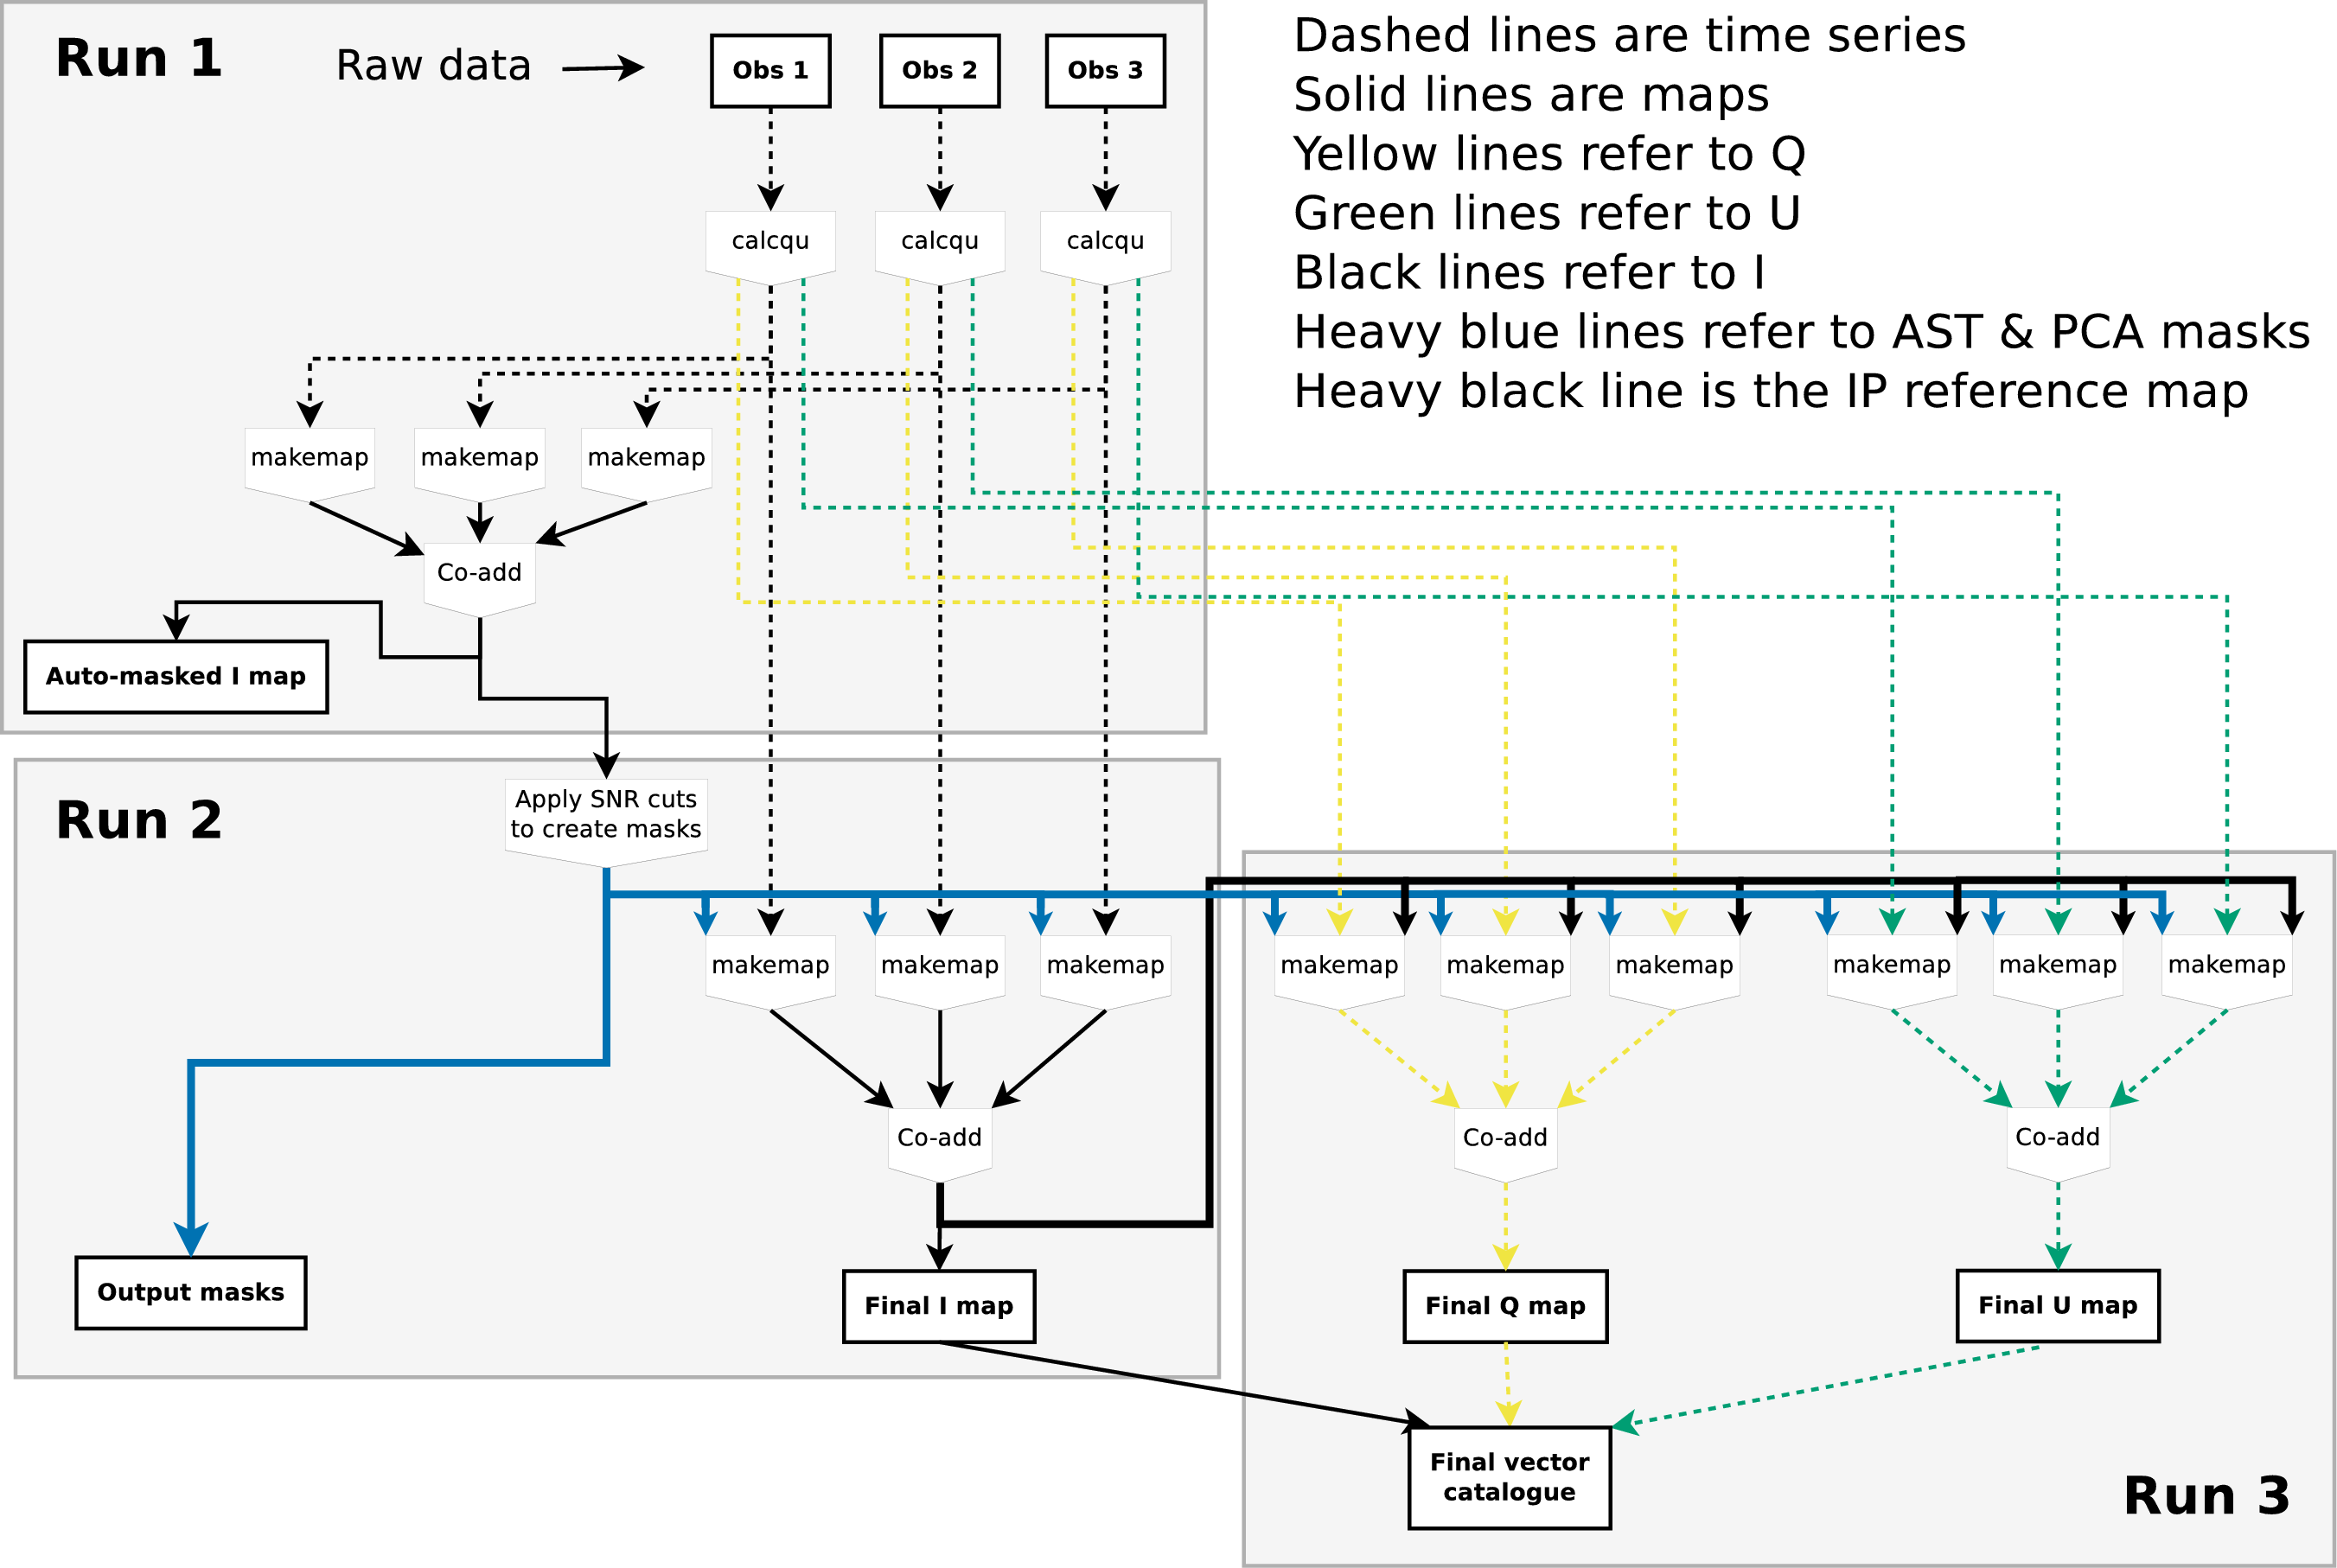
\includegraphics[width=1.0\linewidth]{pol2map_flow}}
\caption [POL-2 Data Flow]{ The data flow of the POL-2 data reduction
  method is presented. In this example, three POL-2 observations are
  reduced and combined in various stages and combination to produce I,
  Q, and U maps and a vector catalogue.  }
\label{fig:pol2drflow}
\end{center}
\end{figure}


\subsection*{Step 1}

The initial step of the process (see Run~1 in \cref{Figure}{fig:pol2drflow}{})
creates a preliminary co-added total intensity
(I) map from the raw data files for all observations provided to the
reduction routine (see \cref{Chapter}{sec:rundr}{}).


\subsubsection*{The process}
The analysed intensity values in the raw data time-streams are first
flat-fielded and converted into Q, U and I time-streams using the
\xref{SMURF:\task{calcqu}}{sun258}{CALCQU} command. These time-streams
are stored for future use in the directory \texttt{qudata}, specified by the
\param{QUDIR} parameter in the example command below.

The \xref{SMURF:makemap}{sun258}{MAKEMAP} command is then used to
create a separate map from the I time-stream for each observation,
using SNR-based ``auto-masking'' to define the background regions that
are to be set to zero at the end of each iteration. This step uses a
PCA threshold of 50 (see \cref{Section}{sec:pca}{PCA} for more details).

\texttt{pca.pcathresh = -50}

These maps are stored for future use in the directory \texttt{maps},
specified by the \param{MAPDIR} parameter. Each map has a name of the form:

\texttt{<UT$\_$DATE>$\_$<OBS$\_$NUM>$\_$<CHUNK$\_$NUM>$\_$imap.sdf}

where \texttt{<CHUNK$\_$NUM>} indicates the raw data file at the start
of the contiguous chunk of data used to create the map, and is usually
0003.

A co-add is then formed by adding all these maps together. Each individual map
is then compared with the co-add, in order to determine a pointing correction
to be applied to the observation in future. These corrections are stored
in the FITS header of the individual maps.


\subsection*{Step 2}

In the second step of the process (see Run~2 in
\cref{Figure}{fig:pol2drflow}{}) an improved I map is produced. These
improvements come from
\begin{enumerate}
\item applying the pointing corrections determined in Step~1
\item the use of an increased number of PCA components
  (\texttt{pca.pcathresh=-150})
\item using a single, fixed mask for all observations. The mask is
  determined from the preliminary co-add I map and thus includes
  fainter structure than would be used if the mask was based on only
  one observation.
\end{enumerate}

\subsection*{Step 3}

In the third step of the reduction process (see Run~3 in
\cref{Figure}{fig:pol2drflow}{}), both the Q and U maps are produced. The production
of the Q and U maps requires the Q and U time-series data (produced in
Step~1), the final I map (produced in Step~2) and the output masks (also
produced in Step~2). Once the Q and U maps are produced a final vector
catalogue is created.

\section{\xlabel{makemap}MAKEMAP}

The POL-2 data reduction builds upon the existing SCUBA-2 Dynamic
Iterative Map-Maker, hereafter just referred to as the ``map-maker". This
is the tool used to produce SCUBA-2 maps, and is invoked by the
\SMURF\ \makemap\ command. It performs some
pre-processing steps to clean the data, solves for multiple signal
components using an iterative algorithm, and bins the resulting
time-series data to produce a final science map.

In \poltwomap\ , the map-maker is used in conjunction with
\xref{calcqu}{sun258}{CALCQU} (see
\cref{Section}{sec:calcqu}{CALCQU}) to produce maps of Q and U, as well as I.

\section{\xlabel{skyloop}SKYLOOP}
\label{sec:skyloop}

An option exists to use the \SMURF\ \skyloop\  command to generate maps
in place of the \SMURF\ \makemap\ command. Each invocation of the
\task{makemap} command creates a single map from the time-series data
for a single observation. If multiple observations are processed together,
multiple invocations of \task{makemap} are used and the resulting maps are
co-added before moving on to the next step, as indicated in
\cref{Figure}{fig:pol2drflow}{}. The \task{skyloop} command, on the other hand,
will process multiple observations in a single invocation, creating a combined
map from all observations. Thus, when using \task{skyloop},
\cref{Figure}{fig:pol2drflow}{} would be effectively changed such that each occurrence
of ``three invocations of \task{makemap} feeding one co-add" would be replaced
by a single invocation of ``\task{skyloop}". See
\cref{Section}{sec:tailoredDR}{Tailoring a reduction}
for more information about the effects of using \task{skyloop}.

\section{\xlabel{calcqu}CALCQU}
\label{sec:calcqu}

In addition to the POL-2 data reduction building on the
existing SCUBA-2 map-maker, \poltwomap\ also relies on the \SMURF\
command \task{CALQU}.

This \xref{calcqu}{sun258}{CALCQU} tool uses time-series files holding Q
and U values from a set of POL-2 time series holding raw data values.
The supplied time-series data files are flat-fielded, cleaned and concatenated,
before being used to establish Q, U and I values for each bolometer. The Q
and U time-series are split into blocks of adjacent time slices. Fits
using these sets of blocks are then used to derive Q, U and I values, and
multiple 2D images are created as the telescope slowly moves across the sky.

Separate Q, U and I estimates are made for each half revolution of the HWP.
The ''Data" values in the returned NDFs are the means of these estimates. If
there are four or more estimates per bolometer, the output will also contain
''Variance" values for each bolometer (which represent the error on
the final mean value, not the variances of the individual values).

\section{\xlabel{pca}PCA}
\label{sec:pca}

One difference between the reduction of SCUBA-2 data and POL-2 data is the
method used to remove the sky background.  The sky background is usually
very large compared with the astronomical signal, and both are subject to
the same form of instrumental polarisation (IP---see
\cref{Section}{sec:ip}{Instrumental Polarisation}). This
IP acting on the high sky background values causes high background values
in the Q and U maps. However, there is evidence that the IP is not
constant across the focal plane, resulting in spatial variations in the
background of the Q and U maps.

For non-POL-2 data, the background is removed using a simple common-mode
model, in which the mean of the bolometer values is found at each time
slice and is then removed from the individual bolometer values. This
ignores any spatial variations in the background, and so fails to remove
the background properly in POL-2 Q and U maps.

To fix this, a second stage of background removal is used when processing
POL-2 data, following the initial common-mode removal. This second stage
is based upon a Principal Component Analysis (PCA) of the 1280
time-streams in each sub-array (the Q and U data are processed
separately). The PCA process identifies the strongest time-dependent
components that are present within multiple bolometers. These components
are assumed to represent the spatially varying background signal and are
removed, leaving just the astronomical signal. The user may specify the number
of components to remove, via a \task{makemap} configuration
parameter called \xparam{PCA.PCATHRESH}{pca.pcathresh} although \poltwomap,
the reduction command for POL-2 data, provides suitable defaults for this parameter.

\begin{itemize}
\item first stage uses \param{pca.pcathresh} = -50
\item second stage uses \param{pca.pcathresh} = -150
\end{itemize}

On each \task{makemap} iteration, the PCA process removes the background (thus
reducing the noise in the map) but also removes some of the astronomical
signal. The amount of astronomical signal removed will be greater for
larger values of \texttt{pca.pcathresh}. However, this astronomical
signal is still present in the original time-series data, and so can be
recovered if sufficient \task{makemap} iterations are performed. In other words,
the use of larger values of \param{pca.pcathresh} slows down the rate at
which astronomical signal is transferred from the time-series data to the
map, thus increasing the number of iterations required to recover the
full astronomical signal in the map.

Spatial variations in the sky background may also be present in non-POL-2
data, but at a lower level. For a discussion of why PCA is not routinely
run on non-polarimetric SCUBA-2 data, see \cref{Appendix}{app:pca}{}.



\section{\xlabel{masking}Masking}
A mask is a two-dimensional array that has the same shape and size as
the final map, and that is used to indicate where the source is
expected to fall within the map. `Bad' pixel values within a mask
indicate background pixels, and `good' pixel values indicate source
pixels. Masks are used for two main purposes:

\begin{enumerate}
\item They prevent the growth of gradients and other artificial large
  scale structures within the map.  For this purpose, the astronomical
  signal at all background pixels defined by the mask is forced to
  zero at the end of each iteration within \task{makemap} (except for the
  final iteration).
\item They prevent bright sources polluting the evaluation of the
  various noise models (PCA, COM, FLT) used within \task{makemap}. Source
  pixels are excluded from the calculation of these models.
\end{enumerate}


The \poltwomap\ script uses different masks for these two purposes---the
``AST'' mask and the ``PCA'' mask.  The PCA mask is, in general, less
extensive than the AST mask, with the source areas being restricted to
the brighter inner regions.  Each of these two masks can either be
generated automatically within \poltwomap, or be specified by a fixed
external NDF.



\section{\xlabel{tailoredDR}Tailoring a reduction}
\label{sec:tailoredDR}

\subsection*{Variances between POL-2 maps}

\param{MAPVAR} is a \poltwomap\ parameter that controls how the variances in the
co-added I, Q, and U maps are formed.

If \param{MAPVAR} is set \texttt{TRUE}, the variances in the co-added I, Q, and U maps
are formed from the spread of pixel data values between the individual
observation maps. If \param{MAPVAR} is \texttt{FALSE} (the default), the variances in
the co-added maps are formed by propagating the pixel variance values
created by \task{makemap} from the individual observation maps (these are
based on the spread of I, Q, or U values that fall within each pixel).

Use \param{MAPVAR}=\texttt{TRUE} only if enough observations are available to make the
variances between them meaningful. A general lower limit on its value
is difficult to define, but a minimum of 10 observations is advised.


If a test of the effect of this option is required on a field for which
the I, Q, and U maps from a set of individual observations are already
available, the following may be done:

\begin{terminalv}
% pol2map in=maps/\* iout=imapvar qout=qmapvar uout=umapvar mapvar=yes \
                   ipcor=no cat=cat_mapvar debias=yes
\end{terminalv}

assuming that the I, Q, and U maps are in directory \file{maps}. The
variances in \file{imapvar.sdf}, \file{qmapvar.sdf} and
\file{umapvar.sdf} will be calculated using the new method, and
these variances will then be used to form the errors in the
\file{cat$\_$mapvar.FIT} catalogue.

In general, within the source regions, the variances created using
\param{MAPVAR}=\texttt{TRUE} will be larger than those created using
using \param{MAPVAR}=\texttt{FALSE} (within background regions there
should be little difference).  This is partly caused by residual
uncorrected pointing errors, which have a particularly large effect near
bright point sources if \param{MAPVAR}=\texttt{TRUE}.

It is also partly caused by intrinisic instabilities within the iterative
map-making algorithm, which allow low-level artifical extended structures
to develop within the source regions defined by the AST mask. Such
artificial structures will vary from observation to observation, and so
will contribute to the variances calculated using \param{MAPVAR}=\texttt{TRUE}.

Two options are provided by \poltwomap\ that may be useful in reducing
the larger-than-expected dispersion between maps made from different
observations:

\begin{enumerate}
\item Setting the parameter \param{OBSWEIGHT}=\texttt{TRUE} when running
\poltwomap\  will cause each observation to be assigned a separate
weight, which will be used when forming the co-add of all observations.
This will affect both the data values and the variances in the resulting
co-add. The purpose of these weights is to down-weight observations that
produce maps that are very dissimilar to maps made from the other observations.

Without this parameter setting, the co-add is formed using weights equal
to the reciprocal of the pixel variance values in each individual
observation's map. As mentioned above, these pixel variance values can
sometimes seriously underestimate the dispersion between observations.
For instance, observations that are clearly bad (e.g. out of focus) can have
relatively low pixel variance values, and thus be included with high weights
in the final co-add.

If the \param{OBSWEIGHT} parameter is set \texttt{TRUE}, each observation
is given an additional weight that is used to factor the per-pixel
weights derived from the pixel variance values, in order to down-weight
observations that are clearly bad. To form these weights, an initial
co-add is formed using equal weights for all observations. The maps made
from the individual observations are then compared with this initial co-add,
and each observation is assigned a weight equal to the reciprocal of the
mean squared residual between the individual observation's map and the
initial co-add (any required pointing correction is applied to the
individual observation map before forming these residuals). The
calculation of the mean squared residual is limited to those pixels
inside the AST mask (i.e. source pixels). The weights derived in this
manner are normalised to have a median value of 1.0, and any normalised
weights larger than 1.0 are reduced to 1.0. An improved co-add is then
formed using these observation weights.

Another iteration is then performed, in which individual maps are compared
with this improved co-add and new weights are derived. This iterative
process continues until the typical error in the middle of the co-add
stops falling significantly.

\item  Setting the parameter \param{SKYLOOP}=\texttt{TRUE} when running
\poltwomap\ will cause maps to be made using the
\xref{SMURF:\task{skyloop}}{sc21}{skyloop} command, instead of
\task{makemap}. In the context of the \task{skyloop} documentation, one
``chunk'' of data usually corresponds to a single observation.

A single invocation of \task{skyloop} creates an I, Q, or U map from all
supplied observations, using a method that attempts to minimise the
intrinsic instabilities of the map-making algorithm within the AST mask.
It should be noted that convergence can require a significantly greater number
of iterations when using \task{skyloop} than when using \task{makemap}. Also,
\task{skyloop} requires much more disk space than \task{makemap}.

The \task{skyloop} command combines all observations together at each
iteration of the map-making algorithm. Since the spurious large-scale
structures created at each iteration are independent of each other,
taking the mean of the maps after each iteration reduces the level of such
structures, and prevents them from growing in amplitude on successive
iterations due to the instability in the map-making algorithm.

\end{enumerate}

The above two methods can be used together by supplying \texttt{TRUE}
values for both \param{OBSWEIGHT} and \param{SKYLOOP}.

\begin{center}
\emph{Note, it is not recommended to use \param{MAPVAR}=\texttt{TRUE} or
\param{SKYLOOP}=\texttt{TRUE} on step 1 (i.e. when creating the auto-masked
maps). Doing so is of no benefit to the final maps and can cause problems
such as negative bowling.}
\end{center}

If the \param{OBSWEIGHT} parameter is used at step 2 or 3, then it must
also be used at step 1.

The following panels show the effects of using \param{SKYLOOP}. and
\param{OBSWEIGHT} on a total intensity mosaic of 21 observations. All
data value maps are shown with a single scaling, and all standard
deviation maps are shown with a single scaling (different from the scaling
for the data value maps):

\newlength{\picwid}
\latexhtml{\setlength{\picwid}{0.3\linewidth}}{\setlength{\picwid}{0.9\linewidth}}

\vspace{5mm}
\begin{tabular}{|ccc|}
\hline
\multicolumn{3}{|c|}{\textbf{SKYLOOP=no OBSWEIGHT=no}} \\
Data value & Std. Dev. (MAPVAR=no) & Std. Dev. (MAPVAR=yes) \\
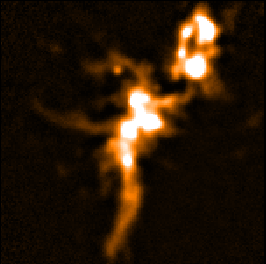
\includegraphics[width=\picwid]{tailoring/i1.png} &
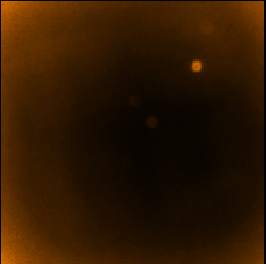
\includegraphics[width=\picwid]{tailoring/sqvar1.png} &
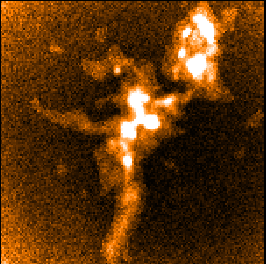
\includegraphics[width=\picwid]{tailoring/disp1.png} \\
\hline
\end{tabular}

\vspace{5mm}
\begin{tabular}{|ccc|}
\hline
\multicolumn{3}{|c|}{\textbf{SKYLOOP=no OBSWEIGHT=yes}} \\
Data value & Std. Dev. (MAPVAR=no) & Std. Dev. (MAPVAR=yes) \\
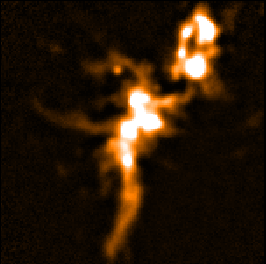
\includegraphics[width=\picwid]{tailoring/i2.png} &
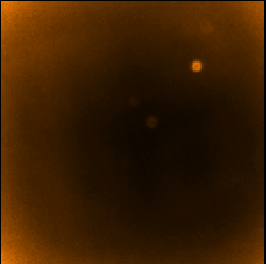
\includegraphics[width=\picwid]{tailoring/sqvar2.png} &
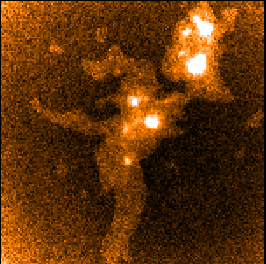
\includegraphics[width=\picwid]{tailoring/disp2.png} \\
\hline
\end{tabular}

\vspace{5mm}
\begin{tabular}{|ccc|}
\hline
\multicolumn{3}{|c|}{\textbf{SKYLOOP=yes OBSWEIGHT=no}} \\
Data value & Std. Dev. (MAPVAR=no) & Std. Dev. (MAPVAR=yes) \\
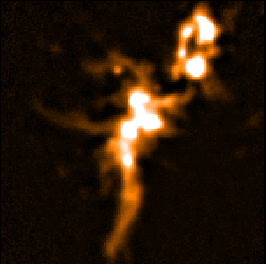
\includegraphics[width=\picwid]{tailoring/i3.png} &
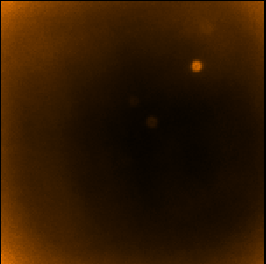
\includegraphics[width=\picwid]{tailoring/sqvar3.png} &
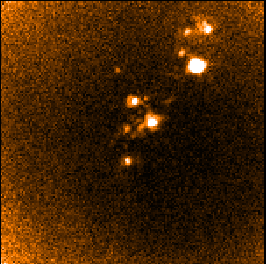
\includegraphics[width=\picwid]{tailoring/disp3.png} \\
\hline
\end{tabular}

\vspace{5mm}
\begin{tabular}{|ccc|}
\hline
\multicolumn{3}{|c|}{\textbf{SKYLOOP=yes OBSWEIGHT=yes}} \\
Data value & Std. Dev. (MAPVAR=no) & Std. Dev. (MAPVAR=yes) \\
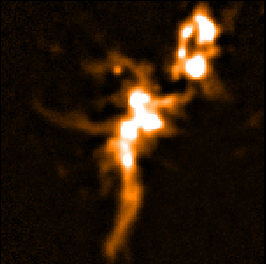
\includegraphics[width=\picwid]{tailoring/i4.png} &
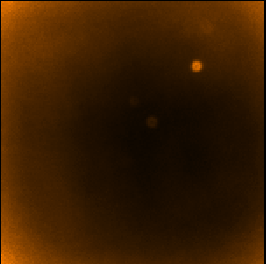
\includegraphics[width=\picwid]{tailoring/sqvar4.png} &
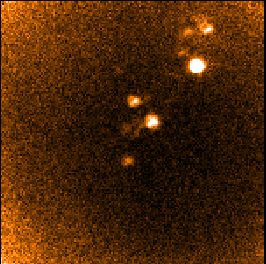
\includegraphics[width=\picwid]{tailoring/disp4.png} \\
\hline
\end{tabular}

\vspace{5mm}

For comparison, below are the equivalent auto-masked maps made by Step~1:

\vspace{5mm}
\begin{tabular}{|ccc|}
\hline
\multicolumn{3}{|c|}{\textbf{Step 1 - auto-masked co-add (SKYLOOP=no OBSWEIGHT=no)}} \\
Data value & Std. Dev. (MAPVAR=no) & Std. Dev. (MAPVAR=yes) \\
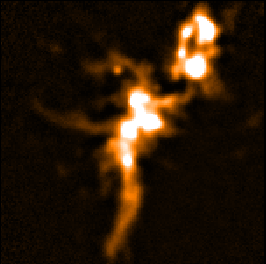
\includegraphics[width=\picwid]{tailoring/i5.png} &
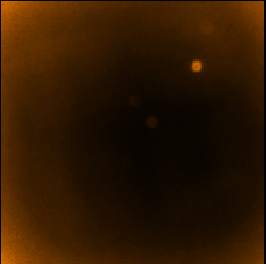
\includegraphics[width=\picwid]{tailoring/sqvar5.png} &
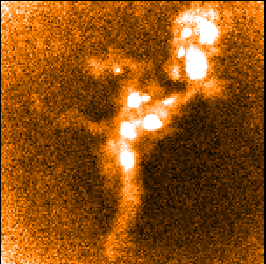
\includegraphics[width=\picwid]{tailoring/disp5.png} \\
\hline
\end{tabular}


